% TikZ source fragment: activation_nonlinearity.tex
% Included by % TikZ source fragment: activation_nonlinearity.tex
% Included by % TikZ source fragment: activation_nonlinearity.tex
% Included by % TikZ source fragment: activation_nonlinearity.tex
% Included by \input{figures/activation_nonlinearity}.
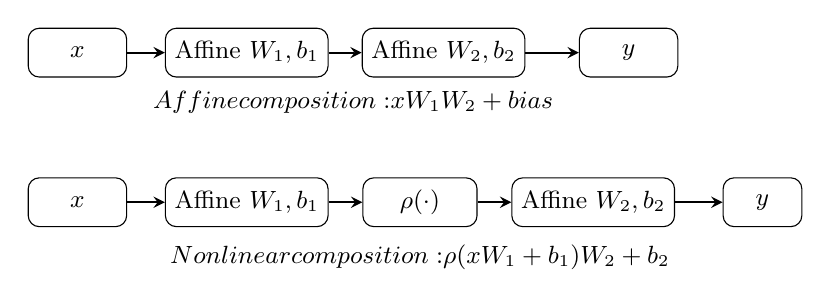
\begin{tikzpicture}[>=stealth, every node/.style={font=\small}]
    \node[draw, rounded corners, minimum width=1.25cm, minimum height=0.62cm]
        (x1) at (0,1.35) {$x$};
    \node[draw, rounded corners, minimum width=1.55cm, minimum height=0.62cm]
        (w11) at (2.15,1.35) {Affine \(W_1,b_1\)};
    \node[draw, rounded corners, minimum width=1.55cm, minimum height=0.62cm]
        (w21) at (4.65,1.35) {Affine \(W_2,b_2\)};
    \node[draw, rounded corners, minimum width=1.25cm, minimum height=0.62cm]
        (y1) at (7.0,1.35) {$y$};
    \draw[->, thick] (x1) -- (w11);
    \draw[->, thick] (w11) -- (w21);
    \draw[->, thick] (w21) -- (y1);
    \node at (3.5,0.72) {\(\text{Affine composition: }xW_1W_2+\text{bias}\)};

    \node[draw, rounded corners, minimum width=1.25cm, minimum height=0.62cm]
        (x2) at (0,-0.55) {$x$};
    \node[draw, rounded corners, minimum width=1.55cm, minimum height=0.62cm]
        (w12) at (2.15,-0.55) {Affine \(W_1,b_1\)};
    \node[draw, rounded corners, minimum width=1.45cm, minimum height=0.62cm]
        (rho) at (4.35,-0.55) {\(\rho(\cdot)\)};
    \node[draw, rounded corners, minimum width=1.55cm, minimum height=0.62cm]
        (w22) at (6.55,-0.55) {Affine \(W_2,b_2\)};
    \node[draw, rounded corners, minimum width=1.0cm, minimum height=0.62cm]
        (y2) at (8.7,-0.55) {$y$};
    \draw[->, thick] (x2) -- (w12);
    \draw[->, thick] (w12) -- (rho);
    \draw[->, thick] (rho) -- (w22);
    \draw[->, thick] (w22) -- (y2);
    \node at (4.35,-1.25)
        {\(\text{Nonlinear composition: }\rho(xW_1+b_1)W_2+b_2\)};
\end{tikzpicture}
.
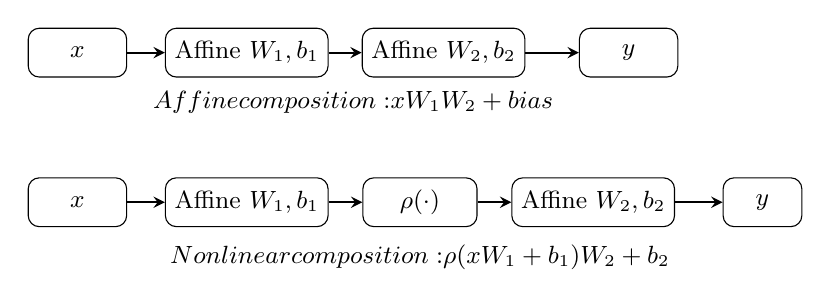
\begin{tikzpicture}[>=stealth, every node/.style={font=\small}]
    \node[draw, rounded corners, minimum width=1.25cm, minimum height=0.62cm]
        (x1) at (0,1.35) {$x$};
    \node[draw, rounded corners, minimum width=1.55cm, minimum height=0.62cm]
        (w11) at (2.15,1.35) {Affine \(W_1,b_1\)};
    \node[draw, rounded corners, minimum width=1.55cm, minimum height=0.62cm]
        (w21) at (4.65,1.35) {Affine \(W_2,b_2\)};
    \node[draw, rounded corners, minimum width=1.25cm, minimum height=0.62cm]
        (y1) at (7.0,1.35) {$y$};
    \draw[->, thick] (x1) -- (w11);
    \draw[->, thick] (w11) -- (w21);
    \draw[->, thick] (w21) -- (y1);
    \node at (3.5,0.72) {\(\text{Affine composition: }xW_1W_2+\text{bias}\)};

    \node[draw, rounded corners, minimum width=1.25cm, minimum height=0.62cm]
        (x2) at (0,-0.55) {$x$};
    \node[draw, rounded corners, minimum width=1.55cm, minimum height=0.62cm]
        (w12) at (2.15,-0.55) {Affine \(W_1,b_1\)};
    \node[draw, rounded corners, minimum width=1.45cm, minimum height=0.62cm]
        (rho) at (4.35,-0.55) {\(\rho(\cdot)\)};
    \node[draw, rounded corners, minimum width=1.55cm, minimum height=0.62cm]
        (w22) at (6.55,-0.55) {Affine \(W_2,b_2\)};
    \node[draw, rounded corners, minimum width=1.0cm, minimum height=0.62cm]
        (y2) at (8.7,-0.55) {$y$};
    \draw[->, thick] (x2) -- (w12);
    \draw[->, thick] (w12) -- (rho);
    \draw[->, thick] (rho) -- (w22);
    \draw[->, thick] (w22) -- (y2);
    \node at (4.35,-1.25)
        {\(\text{Nonlinear composition: }\rho(xW_1+b_1)W_2+b_2\)};
\end{tikzpicture}
.
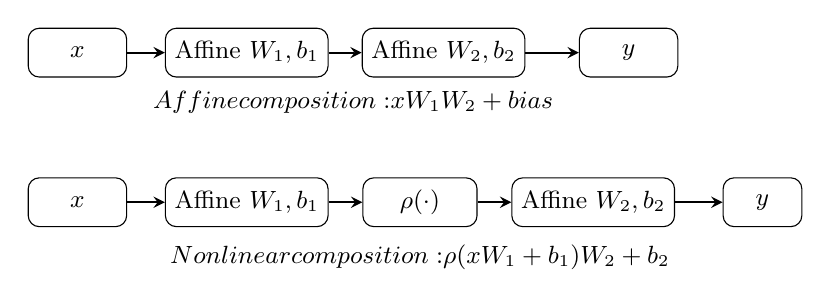
\begin{tikzpicture}[>=stealth, every node/.style={font=\small}]
    \node[draw, rounded corners, minimum width=1.25cm, minimum height=0.62cm]
        (x1) at (0,1.35) {$x$};
    \node[draw, rounded corners, minimum width=1.55cm, minimum height=0.62cm]
        (w11) at (2.15,1.35) {Affine \(W_1,b_1\)};
    \node[draw, rounded corners, minimum width=1.55cm, minimum height=0.62cm]
        (w21) at (4.65,1.35) {Affine \(W_2,b_2\)};
    \node[draw, rounded corners, minimum width=1.25cm, minimum height=0.62cm]
        (y1) at (7.0,1.35) {$y$};
    \draw[->, thick] (x1) -- (w11);
    \draw[->, thick] (w11) -- (w21);
    \draw[->, thick] (w21) -- (y1);
    \node at (3.5,0.72) {\(\text{Affine composition: }xW_1W_2+\text{bias}\)};

    \node[draw, rounded corners, minimum width=1.25cm, minimum height=0.62cm]
        (x2) at (0,-0.55) {$x$};
    \node[draw, rounded corners, minimum width=1.55cm, minimum height=0.62cm]
        (w12) at (2.15,-0.55) {Affine \(W_1,b_1\)};
    \node[draw, rounded corners, minimum width=1.45cm, minimum height=0.62cm]
        (rho) at (4.35,-0.55) {\(\rho(\cdot)\)};
    \node[draw, rounded corners, minimum width=1.55cm, minimum height=0.62cm]
        (w22) at (6.55,-0.55) {Affine \(W_2,b_2\)};
    \node[draw, rounded corners, minimum width=1.0cm, minimum height=0.62cm]
        (y2) at (8.7,-0.55) {$y$};
    \draw[->, thick] (x2) -- (w12);
    \draw[->, thick] (w12) -- (rho);
    \draw[->, thick] (rho) -- (w22);
    \draw[->, thick] (w22) -- (y2);
    \node at (4.35,-1.25)
        {\(\text{Nonlinear composition: }\rho(xW_1+b_1)W_2+b_2\)};
\end{tikzpicture}
.
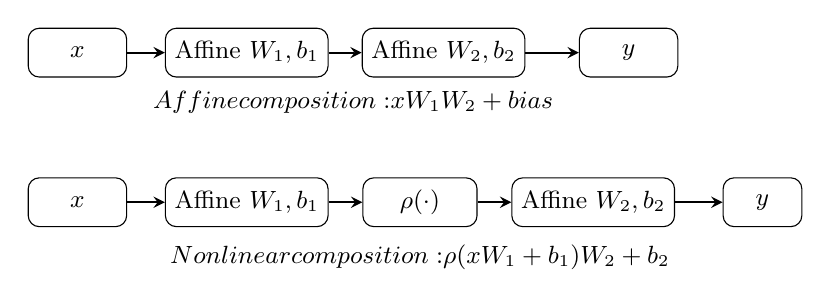
\begin{tikzpicture}[>=stealth, every node/.style={font=\small}]
    \node[draw, rounded corners, minimum width=1.25cm, minimum height=0.62cm]
        (x1) at (0,1.35) {$x$};
    \node[draw, rounded corners, minimum width=1.55cm, minimum height=0.62cm]
        (w11) at (2.15,1.35) {Affine \(W_1,b_1\)};
    \node[draw, rounded corners, minimum width=1.55cm, minimum height=0.62cm]
        (w21) at (4.65,1.35) {Affine \(W_2,b_2\)};
    \node[draw, rounded corners, minimum width=1.25cm, minimum height=0.62cm]
        (y1) at (7.0,1.35) {$y$};
    \draw[->, thick] (x1) -- (w11);
    \draw[->, thick] (w11) -- (w21);
    \draw[->, thick] (w21) -- (y1);
    \node at (3.5,0.72) {\(\text{Affine composition: }xW_1W_2+\text{bias}\)};

    \node[draw, rounded corners, minimum width=1.25cm, minimum height=0.62cm]
        (x2) at (0,-0.55) {$x$};
    \node[draw, rounded corners, minimum width=1.55cm, minimum height=0.62cm]
        (w12) at (2.15,-0.55) {Affine \(W_1,b_1\)};
    \node[draw, rounded corners, minimum width=1.45cm, minimum height=0.62cm]
        (rho) at (4.35,-0.55) {\(\rho(\cdot)\)};
    \node[draw, rounded corners, minimum width=1.55cm, minimum height=0.62cm]
        (w22) at (6.55,-0.55) {Affine \(W_2,b_2\)};
    \node[draw, rounded corners, minimum width=1.0cm, minimum height=0.62cm]
        (y2) at (8.7,-0.55) {$y$};
    \draw[->, thick] (x2) -- (w12);
    \draw[->, thick] (w12) -- (rho);
    \draw[->, thick] (rho) -- (w22);
    \draw[->, thick] (w22) -- (y2);
    \node at (4.35,-1.25)
        {\(\text{Nonlinear composition: }\rho(xW_1+b_1)W_2+b_2\)};
\end{tikzpicture}
